\chapter{Statique des fluides}\label{ch:b1:fluid-statics}

Un sous-marin par trois cents mètres de fond supporte, sur chaque mètre
carré de coque, le poids d'un camion chargé. Un barrage retient un lac
avec un mur épais en bas et mince en haut, pour une raison qui n'a rien
à voir avec la longueur du lac. Un navire de cent mille tonnes flotte
parce qu'il écarte cent mille tonnes d'eau, et s'enfonce d'une main de
plus lorsqu'il passe de la mer dans un fleuve. Tout cela découle d'une
seule relation --- dans un fluide au repos, la pression croît vers le bas
au rythme $\rho g$ --- que ce chapitre établit, applique aux liquides et
à l'atmosphère, et dont il déduit la force sur une paroi ainsi que le
théorème d'Archimède.

\begin{omfigure}
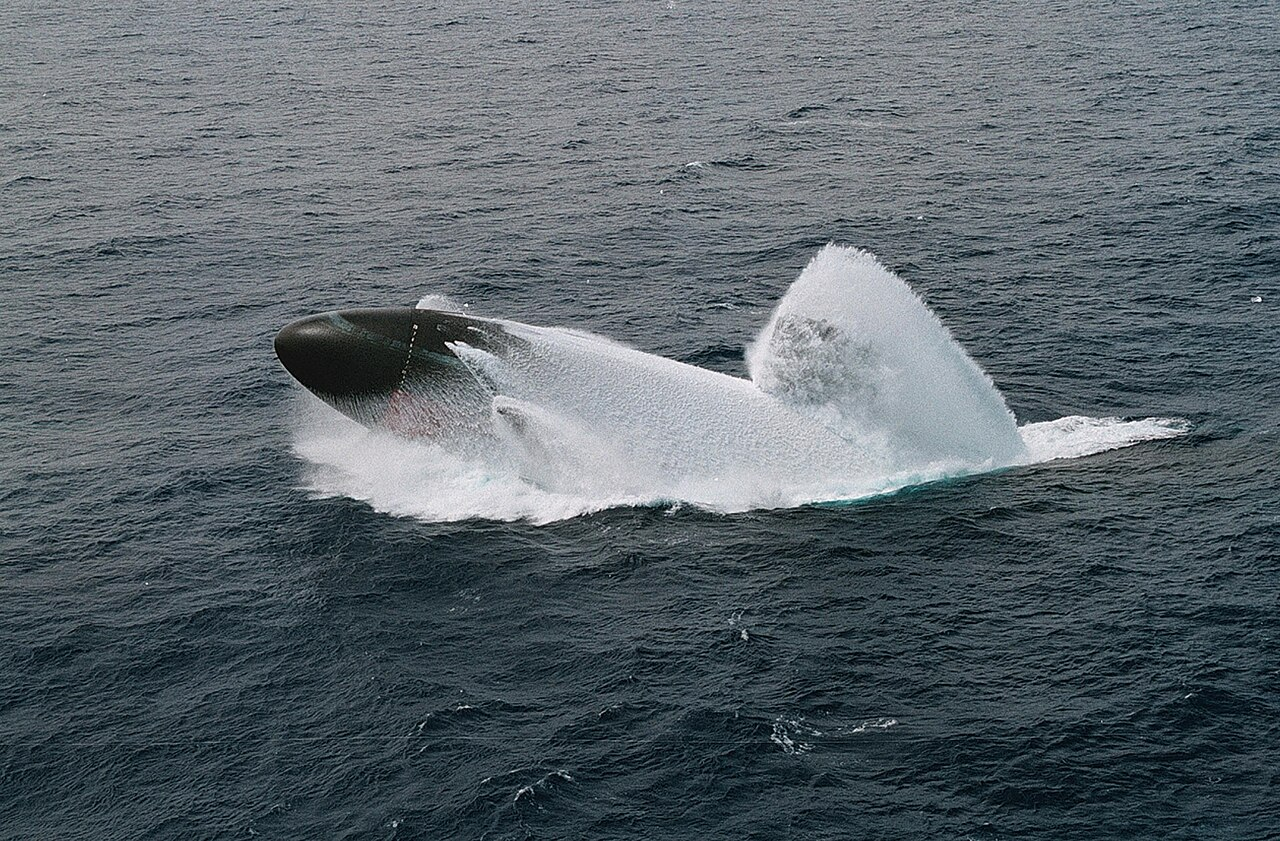
\includegraphics[width=0.60\linewidth]{images/book3/submarine-surfacing.jpg}

{\small Un sous-marin lors d'un exercice de remontée d'urgence (US Navy)~: ses ballasts chassés, il est plus léger que l'eau qu'il déplace et remonte --- le théorème d'Archimède à \qty{7000}{t}.}
\end{omfigure}

\section{La pression dans un fluide au repos}

\begin{proposition}[Isotropie de la pression]\label{prop:b1:fluid-statics:isotropy}
\index{pression!dans un fluide}
Dans un fluide au repos, la force exercée par le fluide sur une petite
surface $\dd S$ placée en un point $M$ vaut $\dd\vect F = P(M)\,\dd S\,\vect n$~:
elle est normale à la surface et dirigée vers elle, et la pression $P(M)$
dépend du point mais \emph{pas} de l'orientation de la surface.
\end{proposition}

\begin{proof}[Démonstration partielle]
Un fluide au repos ne transmet pas de force tangentielle~: la force de
pression est normale, sinon le fluide s'écoulerait. Considérons un petit prisme
triangulaire de fluide autour de $M$, dont les faces ont des orientations
différentes~: il est en équilibre sous les forces de pression sur ses
faces et sous son poids~; le poids varie comme le volume (cube de la
taille) et les forces de pression comme des aires (carré), de sorte que
pour un prisme assez petit seules comptent les forces de pression, et
leur équilibre dans toutes les directions impose le même $P$ sur chaque face.
\end{proof}

\begin{theorem}[Relation fondamentale de la statique des fluides]\label{thm:b1:fluid-statics:fundamental}
\index{relation hydrostatique}
Dans un fluide au repos placé dans le \omterm{prop:b1:newton-dynamics:weight}{champ de pesanteur} uniforme $\vect g = -g\vect e_z$ ($z$
vers le haut), la pression ne dépend que de $z$ et
\[
\frac{\dd P}{\dd z} = -\rho g ,
\]
où $\rho$ est la masse volumique du fluide à ce niveau. La pression croît
vers le bas~; les surfaces d'égale pression (les \emph{isobares}) sont
horizontales, comme l'est la surface libre d'un liquide.
\end{theorem}

\begin{proof}
Considérons une tranche horizontale de fluide, d'aire $S$, comprise entre
$z$ et $z + \dd z$~: elle est poussée vers le haut par $P(z)S$ en dessous,
vers le bas par $P(z + \dd z)S$ au-dessus, et tirée vers le bas par son
poids $\rho gS\,\dd z$. À l'équilibre~:
$P(z)S - P(z + \dd z)S - \rho gS\,\dd z = 0$. Une tranche horizontale ne
subit aucune force horizontale de la pesanteur, donc $P$ est uniforme horizontalement.
\end{proof}

\begin{omfigure}
\begin{tikzpicture}[font=\small, x=1cm, y=1cm]
  \fill[omDef!10] (-2.4,-1.8) rectangle (2.4,1.8);
  \draw[thick, fill=omDef!30] (-1.2,-0.25) rectangle (1.2,0.25);
  \draw[-Stealth, omThm, very thick] (0,-1.3) -- (0,-0.3) node[pos=0.0, below] {$P(z)\,S$};
  \draw[-Stealth, omThm, very thick] (0,1.3) -- (0,0.3) node[pos=0.0, above] {$P(z + \dd z)\,S$};
  \draw[-Stealth, omProp, very thick] (0.9,0) -- (0.9,-0.9) node[right] {$\rho gS\,\dd z$};
  \draw[Stealth-Stealth] (-1.5,-0.25) -- (-1.5,0.25) node[midway, left] {$\dd z$};
  \draw[-Stealth] (2.8,-1.5) -- (2.8,1.5) node[above] {$z$};
  \node[font=\footnotesize] at (0,-2.1) {$P(z) - P(z + \dd z) = \rho g\,\dd z$};
\end{tikzpicture}\qquad
\begin{tikzpicture}[font=\small, x=1cm, y=1cm]
  % communicating vessels
  \fill[omDef!25] (0,0) rectangle (0.8,2.4); \fill[omDef!25] (0,0) rectangle (4.2,0.6); \fill[omDef!25] (1.8,0) rectangle (2.4,2.4); \fill[omDef!25] (3.4,0) rectangle (4.2,2.4);
  \draw[thick] (0,3.2) -- (0,0) -- (4.2,0) -- (4.2,3.2); \draw[thick] (0.8,3.2) -- (0.8,0.6) -- (1.8,0.6) -- (1.8,3.2); \draw[thick] (2.4,3.2) -- (2.4,0.6) -- (3.4,0.6) -- (3.4,3.2);
  \draw[omDef, thick] (0,2.4) -- (0.8,2.4); \draw[omDef, thick] (1.8,2.4) -- (2.4,2.4); \draw[omDef, thick] (3.4,2.4) -- (4.2,2.4);
  \draw[dashed, omThm] (-0.3,2.4) -- (4.5,2.4); \node[omThm, right] at (4.5,2.4) {même niveau};
  \node[font=\footnotesize] at (2.1,-0.4) {même $P$ sur une horizontale};
\end{tikzpicture}

{\small À gauche~: équilibre d'une tranche horizontale de fluide --- la
pression en dessous doit dépasser celle du dessus du poids de la tranche
par unité d'aire. À droite~: vases communicants --- une horizontale
rencontre partout la même pression dans un liquide connexe, de sorte que
les surfaces libres se placent au même niveau quelles que soient les formes.}
\end{omfigure}

\begin{corollary}[Fluide incompressible]\label{cor:b1:fluid-statics:incompressible}
\index{pression hydrostatique}
Dans un liquide de masse volumique uniforme $\rho$, la pression à la
profondeur $h$ sous un point où elle vaut $P_0$ est
\[
P = P_0 + \rho gh .
\]
Eau~: \qty{1}{bar} de plus tous les \qty{10}{m}. Deux points d'un liquide
connexe situés au même niveau sont à la même pression~; les surfaces
libres de vases communicants se placent au même niveau~; une pression
appliquée en un point quelconque d'un liquide enfermé se transmet
intégralement à tous les autres (principe de Pascal).
\end{corollary}

\begin{proof}
Il suffit d'intégrer $\dd P/\dd z = -\rho g$ à $\rho$ constant~; le reste
tient à l'horizontalité des isobares et à l'unicité de $P$ sur un niveau.
\end{proof}

\begin{example}[Manomètres et presses]\label{ex:b1:fluid-statics:manometer}
\index{manomètre}\index{presse hydraulique}
Un tube en U rempli de mercure ($\rho = \qty{13600}{kg/m^3}$) dont les
colonnes diffèrent de $h = \qty{760}{mm}$ mesure une différence de pression
$\rho gh = \qty{1.013e5}{Pa}$
--- l'atmosphère, qui soutient une colonne d'eau de \qty{10.3}{m}. Une
\omterm{ex:b1:fluid-statics:manometer}{presse hydraulique}~: une force $F_1$ sur un piston d'aire $S_1$ élève la
pression de $F_1/S_1$ partout~; sur le grand piston $S_2$ elle donne
$F_2 = F_1S_2/S_1$ --- cinquante fois plus pour cinquante fois l'aire, au
prix d'une course cinquante fois plus courte (l'énergie se conserve~: $F_1d_1 = F_2d_2$).
\end{example}

\section{L'atmosphère}

\begin{proposition}[Atmosphère isotherme]\label{prop:b1:fluid-statics:atmosphere}
\index{formule barométrique}\index{hauteur d'échelle}
Pour un \omterm{def:b1:kinetic-theory:model}{gaz parfait} de masse molaire $M$ à température uniforme $T$ dans
un \omterm{prop:b1:newton-dynamics:weight}{champ de pesanteur} uniforme,
\[
P(z) = P_0\,\eu^{-z/H}, \qquad H = \frac{RT}{Mg} ,
\]
la \emph{\omterm{prop:b1:fluid-statics:atmosphere}{hauteur d'échelle}}~: environ \qty{8}{km} pour l'air~; la pression
est divisée par deux tous les $H\ln2 \approx \qty{5.5}{km}$.
\end{proposition}

\begin{proof}
$\rho = PM/RT$ (équation d'état), donc $\dd P/\dd z = -(Mg/RT)P$~: une
équation différentielle linéaire du premier ordre, $P = P_0\eu^{-Mgz/RT}$.
\end{proof}

\begin{example}[L'air raréfié]\label{ex:b1:fluid-statics:altitude}
Avec $T = \qty{260}{K}$ (une moyenne sur la basse atmosphère), $H =
\qty{7.6}{km}$~: $P = 0.52P_0$ à \qty{5000}{m}, $0.31P_0$ au sommet de
l'Everest --- proche des valeurs mesurées $0.54$ et $0.33$~; l'atmosphère
réelle se refroidit avec l'altitude, ce dont le volume de deuxième année
tient compte. Le modèle dit aussi pourquoi la mer est différente~: l'eau
est huit cents fois plus dense et presque incompressible, de sorte que sa
pression croît linéairement, d'un bar tous les dix mètres, sans \omterm{prop:b1:fluid-statics:atmosphere}{hauteur d'échelle}.
\end{example}

\begin{omfigure}
\begin{tikzpicture}
\begin{axis}[omaxis, axis x line=bottom, axis y line=left, width=8cm, height=5.4cm, xlabel={$z$ (\unit{km})}, ylabel={$P/P_0$},
    xlabel style={at={(axis description cs:0.5,-0.12)}, anchor=north},
    xmin=0, xmax=30, ymin=0, ymax=1.1, xtick={5.5,10,20,30}, xticklabels={$5.5$,$10$,$20$,$30$}, ytick={0.5,1}]
  \addplot[omDef, thick, domain=0:30, samples=100] {exp(-x/7.6)};
  \draw[dashed, omExo] (axis cs:0,0.5) -- (axis cs:5.3,0.5) -- (axis cs:5.3,0);
  \node[omDef, font=\footnotesize] at (axis cs:16,0.45) {$P_0\eu^{-z/H}$, $H = \qty{7.6}{km}$};
\end{axis}
\end{tikzpicture}

{\small L'atmosphère isotherme~: la pression (et la masse volumique)
décroissent exponentiellement avec l'altitude, divisées par deux tous les
\qty{5.5}{km}. Neuf dixièmes de l'air se trouvent au-dessous de \qty{17}{km}.}
\end{omfigure}

\section{Forces sur les parois}

\begin{proposition}[Force sur une paroi verticale]\label{prop:b1:fluid-statics:wall}
\index{centre de poussée}
Un liquide de profondeur $h$ contre une paroi verticale rectangulaire de
largeur $L$ (la pression atmosphérique agissant sur les deux faces et se
compensant) exerce la force horizontale
\[
F = \tfrac12\rho gh^2L ,
\]
équivalente à une force unique appliquée au \emph{\omterm{prop:b1:fluid-statics:wall}{centre de poussée}}, à
la profondeur $2h/3$ --- la résultante s'exerce bas, là où la pression est
la plus grande.
\end{proposition}

\begin{proof}
À la profondeur $x$ la pression relative vaut $\rho gx$~; sur la bande de
hauteur $\dd x$ la force vaut $\rho gxL\,\dd x$~; on intègre de $0$ à $h$. Son
moment par rapport à la ligne de surface vaut $\int_0^h\rho gx^2L\,\dd x = \tfrac13\rho gh^3L$~;
en divisant par $F$, on obtient le \omterm{def:b1:angular-momentum:moment}{bras de levier} $2h/3$.
\end{proof}

\begin{omfigure}
\begin{tikzpicture}[font=\small, x=1cm, y=1cm]
  \fill[omDef!20] (-3.6,0) rectangle (0,2.8);
  \draw[thick] (-3.8,2.8) -- (0,2.8); \draw[omDef, thick] (-3.6,2.8) -- (0,2.8);
  \draw[thick, fill=omExo!40] (0,0) -- (0,3.2) -- (1.0,3.2) -- (1.8,0) -- cycle;
  \draw[thick] (-3.8,0) -- (2.6,0);
  \foreach \y/\l in {2.5/0.15, 2.0/0.4, 1.5/0.65, 1.0/0.9, 0.5/1.15, 0.1/1.35} {\draw[-Stealth, omThm] (-\l,\y) -- (0,\y);}
  \draw[omThm, dashed] (0,2.8) -- (-1.4,0);
  \draw[-Stealth, omThm, very thick] (-2.6,0.93) -- (-0.05,0.93) node[pos=0.0, left] {$F = \tfrac12\rho gh^2L$};
  \draw[Stealth-Stealth] (2.2,2.8) -- (2.2,0.93) node[midway, right] {$\tfrac23 h$};
  \draw[Stealth-Stealth] (-3.2,2.8) -- (-3.2,0) node[midway, left] {$h$};
\end{tikzpicture}

{\small La pression sur un barrage croît linéairement avec la profondeur
(flèches), de sorte que la résultante s'applique aux deux tiers de la
profondeur~: le mur doit être le plus épais en bas. La force ne dépend
que de $h$ et de $L$, non de la quantité d'eau retenue derrière.}
\end{omfigure}

\begin{example}[Un barrage]\label{ex:b1:fluid-statics:dam}
$h = \qty{20}{m}$, $L = \qty{100}{m}$~: $F = \tfrac12 \times 1000 \times 9.81 \times
400 \times 100 = \qty{2.0e8}{N}$ --- vingt mille tonnes, appliquées
\qty{13}{m} sous la surface, et cela que le lac derrière soit une mare ou
un fjord~: c'est le \emph{paradoxe hydrostatique}.
\end{example}

\section{Le théorème d'Archimède}

\begin{theorem}[Archimède]\label{thm:b1:fluid-statics:archimedes}
\index{théorème d'Archimède}\index{poussée d'Archimède}\index{centre de carène}
Un corps immergé dans un fluide au repos subit, de la part des forces de
pression, une résultante --- la \emph{\omterm{thm:b1:fluid-statics:archimedes}{poussée d'Archimède}} --- égale et
opposée au poids du fluide qu'il déplace,
\[
\vect\Pi = -\rho_{\text{fluid}}V_{\text{immersed}}\,\vect g ,
\]
appliquée au \omterm{def:b1:systems-of-points:cm}{centre de masse} du fluide déplacé (le \emph{\omterm{thm:b1:fluid-statics:archimedes}{centre de
carène}}).
\end{theorem}

\begin{proof}
Les forces de pression sur la surface du corps ne dépendent que de la
forme de cette surface et du fluide qui l'entoure. Remplaçons le corps,
par la pensée, par du fluide au repos occupant le même volume~: ce fluide
est en équilibre sous son poids et sous ces mêmes forces de pression, donc
les forces de pression équilibrent son poids --- leur somme vaut
$-\rho V\vect g$, appliquée en son \omterm{def:b1:systems-of-points:cm}{centre de masse}. Supprimons l'expérience
de pensée~: les forces de pression, elles, n'ont pas changé.
\end{proof}

\begin{corollary}[Flottaison]\label{cor:b1:fluid-statics:floating}
\index{flottaison}
Un corps de masse volumique $\rho_b$ flotte dans un fluide de masse
volumique $\rho_f > \rho_b$ avec la fraction $\rho_b/\rho_f$ de son volume
immergée~; si $\rho_b >
\rho_f$, il coule, avec un poids apparent $(\rho_b - \rho_f)Vg$.
\end{corollary}

\begin{proof}
Le poids $\rho_bVg$ égale la poussée $\rho_fV_{\text{imm}}g$.
\end{proof}

\begin{omfigure}
\begin{tikzpicture}[font=\small, x=1cm, y=1cm]
  \fill[omDef!15] (-3.6,-2.2) rectangle (3.6,0);
  \draw[omDef, thick] (-3.6,0) -- (3.6,0);
  % iceberg-like block: rectangle 2 x 1.6, 90% immersed
  \draw[thick, fill=white] (-1.0,-1.44) rectangle (1.0,0.16);
  \fill (0,-0.64) circle (1.5pt) node[right] {$G$};
  \fill[omDef] (0,-0.72) circle (1.5pt) node[left] {$C$};
  \draw[-Stealth, omThm, very thick] (0,-0.64) -- (0,-1.9) node[below] {$\rho_bVg$};
  \draw[-Stealth, omDef, very thick] (0,-0.72) -- (0,0.55) node[above] {$\rho_fV_{\text{imm}}g$};
  \node[font=\footnotesize] at (2.4,-1.2) {$\dfrac{V_{\text{imm}}}{V} = \dfrac{\rho_b}{\rho_f}$};
\end{tikzpicture}

{\small Un corps flottant~: son poids, appliqué en son \omterm{def:b1:systems-of-points:cm}{centre de masse} $G$,
équilibre la \omterm{thm:b1:fluid-statics:archimedes}{poussée d'Archimède}, appliquée au \omterm{thm:b1:fluid-statics:archimedes}{centre de carène} $C$ (le
centre du volume immergé). De la glace ($\rho = \qty{917}{kg/m^3}$) dans
l'eau de mer ($\qty{1025}{kg/m^3}$)~: $89\%$ sous la surface.}
\end{omfigure}

\begin{example}[Trois poussées]\label{ex:b1:fluid-statics:buoy}
Un densimètre est un tube lesté qui s'enfonce jusqu'à déplacer son propre
poids~: plus le liquide est dense, moins il s'enfonce --- une mesure de
masse volumique lue sur sa tige. Un ballon de \qty{2800}{m^3} d'air chaud
à \qty{373}{K} déplace \qty{3.4}{t} d'air froid et pèse \qty{2.6}{t} d'air
chaud~: \qty{0.7}{t} de force ascensionnelle (\cref{pb:b1:kinetic-theory:1}).
Un navire de \qty{100000}{t} déplace \qty{97600}{m^3} d'eau de mer~; en eau
douce ($\qty{1000}{kg/m^3}$) il doit en déplacer $2.5\%$ de plus et
s'enfonce davantage --- d'où les marques de franc-bord sur sa coque.
\end{example}

\begin{remark}[Stabilité]\label{rem:b1:fluid-statics:stability}
\index{métacentre}
Un corps flottant incliné d'un petit angle est redressé si la \omterm{thm:b1:fluid-statics:archimedes}{poussée
d'Archimède}, désormais appliquée au centre déplacé du nouveau volume
immergé, produit un moment de redressement --- ce qui se produit lorsque
le \emph{métacentre} (le point où la ligne d'action de la poussée coupe
l'axe du corps) se trouve au-dessus de $G$. Du lest bas dans la coque
abaisse $G$ et stabilise le navire~; un bateau trop lourd du haut chavire.
\end{remark}

\section{Exercices}

\begin{exercise}[$\star$]\label{exo:b1:fluid-statics:1}
Pression absolue à \qty{10}{m}, \qty{100}{m} et \qty{1}{km} sous la mer
($\rho = \qty{1025}{kg/m^3}$)~; force sur un hublot de \qty{1.0}{m^2} à
\qty{300}{m}.
\end{exercise}

\begin{exercise}[$\star$]\label{exo:b1:fluid-statics:2}
Hauteur d'une colonne de mercure qui équilibre \qty{1.013e5}{Pa}~; celle
d'une colonne d'eau. Pourquoi une pompe aspirante n'élève-t-elle pas l'eau
de plus de \qty{10}{m} environ~?
\end{exercise}

\begin{exercise}[$\star$]\label{exo:b1:fluid-statics:3}
Un cric hydraulique~: \qty{100}{N} sur un piston de \qty{2.0}{cm^2}, charge
soulevée sur un piston de \qty{200}{cm^2}~; course de chacun si le petit
piston parcourt \qty{20}{cm}.
\end{exercise}

\begin{exercise}[$\star$]\label{exo:b1:fluid-statics:4}
Un tube en U contient de l'eau~; on verse de l'huile ($\rho = \qty{850}{kg/m^3}$)
dans une branche, où elle forme une colonne de \qty{12}{cm}. Dénivelé entre
les deux surfaces libres.
\end{exercise}

\begin{exercise}[$\star\star$]\label{exo:b1:fluid-statics:5}
\omterm{prop:b1:fluid-statics:atmosphere}{Hauteur d'échelle} de l'atmosphère à \qty{273}{K}~; pression à \qty{5000}{m}
et à \qty{8848}{m}~; altitude à laquelle $P = P_0/2$. Comparer avec les
valeurs citées au \cref{ch:b1:kinetic-theory}.
\end{exercise}

\begin{exercise}[$\star\star$]\label{exo:b1:fluid-statics:6}
Un barrage rectangulaire de \qty{100}{m} de large retient \qty{20}{m} d'eau.
Force totale, profondeur du \omterm{prop:b1:fluid-statics:wall}{centre de poussée} et moment de l'eau par
rapport au pied du barrage. Pourquoi un barrage est-il courbé vers l'eau~?
\end{exercise}

\begin{exercise}[$\star\star$]\label{exo:b1:fluid-statics:7}
Fraction d'un iceberg immergée (glace \qty{917}{kg/m^3}, eau de mer
\qty{1025}{kg/m^3})~; d'une bûche de masse volumique \qty{600}{kg/m^3} en eau
douce~; combien de personnes de \qty{75}{kg} un radeau de \qty{2.0}{m^3} de
ce bois peut-il porter avant que son plancher ne soit au ras de l'eau~?
\end{exercise}

\begin{exercise}[$\star\star$]\label{exo:b1:fluid-statics:8}
Un densimètre de masse \qty{20}{g}, dont la tige a une section de
\qty{0.50}{cm^2}, flotte dans l'eau en laissant émerger \qty{4.0}{cm} de tige.
Quelle longueur de tige émerge dans une saumure de masse volumique
\qty{1100}{kg/m^3}~? Sensibilité (en centimètres par unité de densité)~?
\end{exercise}

\begin{exercise}[$\star\star$]\label{exo:b1:fluid-statics:9}
Un sous-marin de \qty{3000}{m^3} a une masse de \qty{2800}{t} ballasts vides.
Fraction émergée en surface (eau de mer)~; masse d'eau à embarquer pour une
flottabilité nulle~; que se passe-t-il s'il entre ensuite dans un estuaire
d'eau douce~?
\end{exercise}

\begin{exercise}[$\star\star\star$]\label{exo:b1:fluid-statics:10}
Un ballon d'enfant contient \qty{10}{L} d'hélium ($M = \qty{4}{g/mol}$) à
\qty{1}{bar} et \qty{293}{K}~; le caoutchouc pèse \qty{3.0}{g}. Force
ascensionnelle nette~; masse de ficelle qu'il peut porter.
\end{exercise}

\begin{exercise}[$\star\star\star$]\label{exo:b1:fluid-statics:11}
Démontrer que le \omterm{prop:b1:fluid-statics:wall}{centre de poussée} sur une paroi verticale rectangulaire se
trouve à $2h/3$ en calculant le moment des forces de pression par rapport à
la ligne de surface. Où se trouve-t-il pour une paroi qui n'est immergée que
partiellement, disons de la profondeur $h_1$ à $h_2$~?
\end{exercise}

\begin{exercise}[$\star\star\star$]\label{exo:b1:fluid-statics:12}
Un densimètre cylindrique (masse $m$, section $S$) qui flotte dans un
liquide de masse volumique $\rho$ est enfoncé de $x$ puis lâché. Montrer
qu'il oscille harmoniquement et donner la période~; la calculer pour $m =
\qty{20}{g}$, $S = \qty{0.50}{cm^2}$, dans l'eau. (\cref{ex:b1:oscillators-resonance:bob}
revisité.)
\end{exercise}

\begin{omfigure}
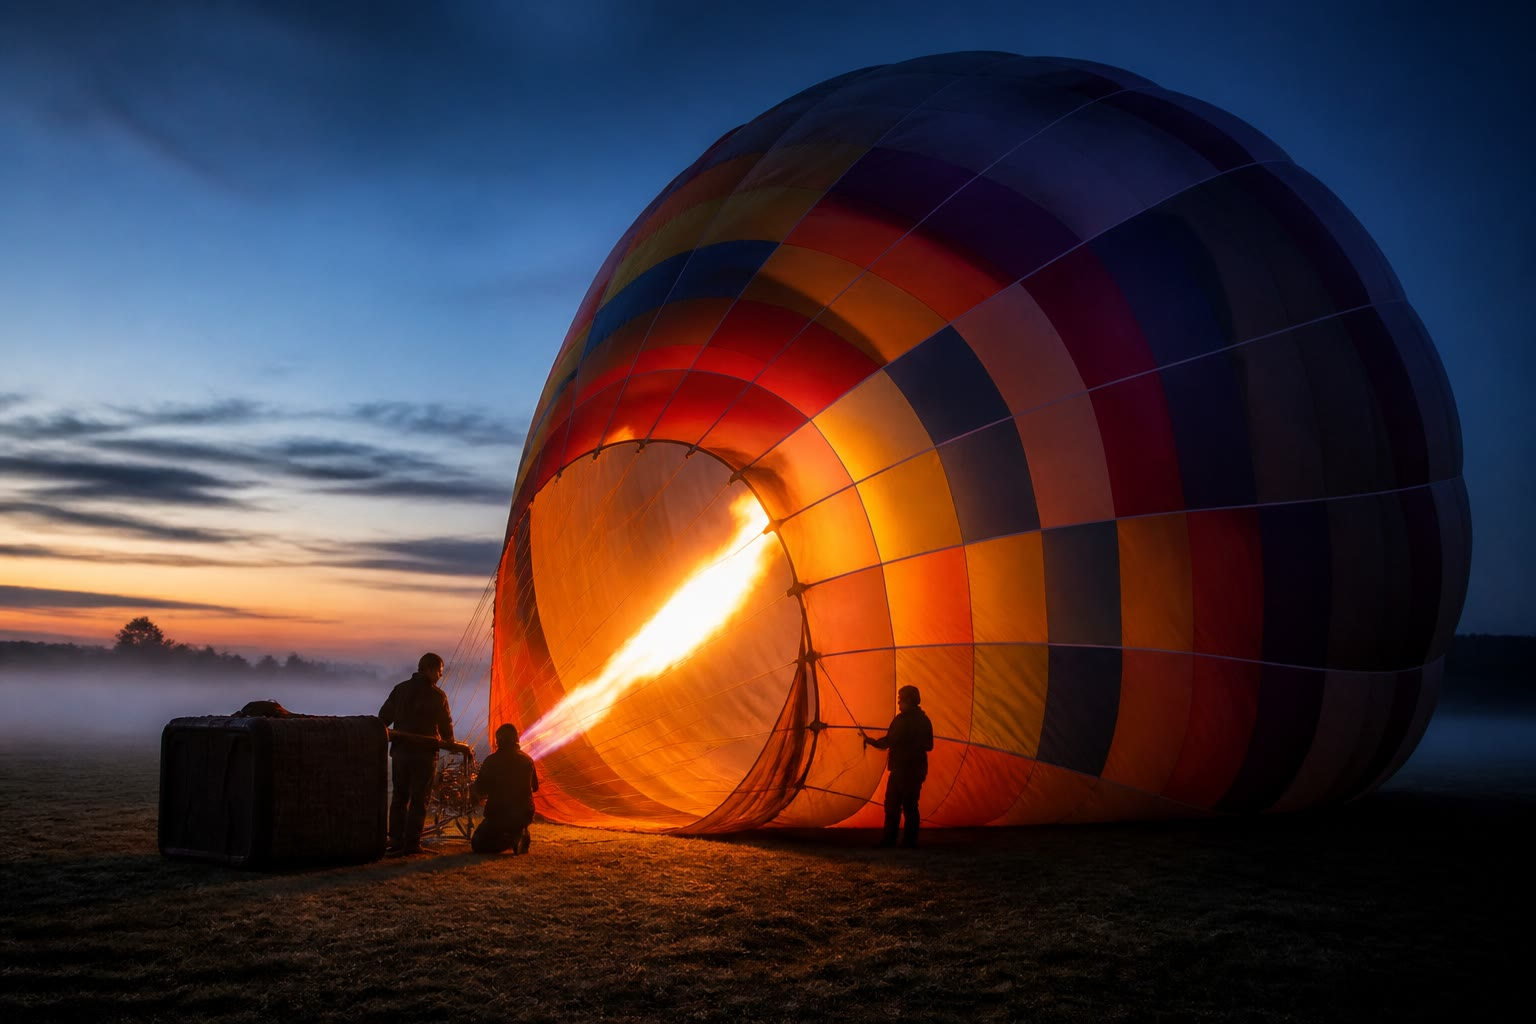
\includegraphics[width=0.58\linewidth]{images/book3/ai/b3-20-hot-air-balloon-burner.jpg}

{\small Gonflage d'une montgolfière~: l'air chauffé est moins dense que l'air froid qui l'entoure, et la \omterm{thm:b1:fluid-statics:archimedes}{poussée d'Archimède} sur l'enveloppe l'emporte sur son poids.}
\end{omfigure}

\section{Problème~: le sous-marin}

\begin{problem}[{Problème du week-end --- une coque d'acier par trois
cents mètres de fond~: la pression sur ses tôles, l'eau qu'elle doit
avaler pour plonger et chasser pour remonter, la plongeuse qui la quitte
et le pétrolier qui passe au-dessus}]
\label{pb:b1:fluid-statics:1}
Eau de mer~: $\rho = \qty{1025}{kg/m^3}$~; eau douce \qty{1000}{kg/m^3}~;
$P_0 = \qty{1.013e5}{Pa}$~; $g = \qty{9.81}{m/s^2}$. La coque du sous-marin
enferme $V = \qty{3000}{m^3}$~; ballasts vides, sa masse vaut
$m_0 = \qty{2800}{t}$.

\medskip
\noindent\textbf{Partie I --- La pression sur la coque.}
\begin{enumerate}
  \item Pression absolue à \qty{300}{m}, en \omterm{def:b1:kinetic-theory:pressure}{pascals} et en bars.
  \item Force sur un panneau circulaire de \qty{0.80}{m} de diamètre à cette
        profondeur~; comparer au poids d'un camion.
  \item Force sur un mètre carré de coque à la quille si la coque mesure
        \qty{10}{m} de haut et que son sommet est à \qty{300}{m}~: quel écart
        avec le sommet~?
  \item L'eau est légèrement compressible ($\chi_T = \qty{4.6e-10}{Pa^{-1}}$)~:
        de quelle fraction l'eau de mer est-elle plus dense à \qty{300}{m}
        qu'en surface~? Cela change-t-il la pression calculée plus haut~?
  \item L'équipage respire de l'air à \qty{1}{atm}~: pourquoi la coque
        doit-elle être un cylindre épais, et pourquoi un cylindre résiste-t-il
        mieux qu'une boîte à faces planes~?
  \item Une coque cylindrique mince de rayon $R$ et d'épaisseur $e$ soumise
        à une surpression extérieure $\Delta P$ supporte dans sa paroi une
        contrainte de compression $\Delta P\,R/e$. Pour $R = \qty{5.0}{m}$ et
        $e = \qty{3.0}{cm}$ à \qty{300}{m}, la calculer et la comparer à la
        limite d'élasticité de l'acier, environ \qty{600}{MPa}.
\end{enumerate}

\medskip
\noindent\textbf{Partie II --- Plonger et flotter.}
\begin{enumerate}[resume]
  \item En surface, ballasts vides, quel volume de la coque émerge~?
  \item Quelle masse d'eau de mer les ballasts doivent-ils embarquer pour
        que le sous-marin reste entre deux eaux (flottabilité nulle)~?
  \item En équilibre à \qty{300}{m}, la coque est comprimée de $0.1\%$ par
        la pression. Calculer la force résultante et dire si l'équilibre est
        stable vis-à-vis de la profondeur.
  \item En flottabilité nulle, le bâtiment passe de la mer dans un estuaire
        d'eau douce. Force résultante~? Dans quel sens part-il, et que doit
        faire l'équipage~?
  \item On tire une torpille de \qty{20}{t}. Que doit faire immédiatement le
        système de ballasts, et de combien~?
  \item Pourquoi un sous-marin chasse-t-il ses ballasts à l'air comprimé, et
        pourquoi la pression de cet air limite-t-elle la profondeur à
        laquelle il peut le faire~?
  \item Estimer le volume d'air à \qty{1}{atm} nécessaire pour vider
        \qty{275}{m^3} de ballasts à \qty{300}{m} (loi de Boyle--Mariotte,
        $PV$ constant).
\end{enumerate}

\medskip
\noindent\textbf{Partie III --- La plongeuse.}
Une plongeuse quitte la surface avec \qty{6.0}{L} d'air dans les poumons.
\begin{enumerate}[resume]
  \item Pression absolue à \qty{10}{m} et à \qty{30}{m}.
  \item Si elle descend en apnée, quel est le volume de ses poumons à
        \qty{30}{m}~?
  \item Une plongeuse en scaphandre respire de l'air à la pression ambiante
        à \qty{30}{m} et remonte en bloquant sa respiration~: volume qu'il
        faudrait à ses poumons en surface, et la leçon à en tirer.
  \item Un tuba de \qty{1.0}{m} de long~: différence de pression entre l'eau
        qui presse la poitrine de la plongeuse et l'air de ses poumons~;
        force sur une poitrine de \qty{0.05}{m^2}~; peut-elle inspirer~?
  \item La bouteille contient \qty{12}{L} à \qty{200}{bar}~: combien de litres
        d'air cela fait-il à \qty{30}{m}, et pour combien de temps à
        \qty{20}{L} par minute~?
\end{enumerate}

\medskip
\noindent\textbf{Partie IV --- Le pétrolier au-dessus.}
\begin{enumerate}[resume]
  \item Un pétrolier de \qty{100000}{t} flotte en eau de mer~: volume d'eau
        déplacé.
  \item Son aire de flottaison vaut \qty{8000}{m^2}~: de combien monte-t-il
        ou s'enfonce-t-il en entrant en eau douce~?
  \item Chargement de \qty{10000}{t} de pétrole~: variation du tirant d'eau.
  \item Vide, le pétrolier a un \omterm{def:b1:systems-of-points:cm}{centre de masse} haut~; il embarque alors de
        l'eau de mer en ballast. Pourquoi, en termes de métacentre~?
  \item La coque du pétrolier à sa quille (tirant d'eau \qty{20}{m})~:
        pression et force par mètre carré, comparées à celles du sous-marin
        à \qty{300}{m}.
  \item Le pétrolier passe exactement au-dessus du sous-marin. Celui-ci
        ressent-il ses \qty{100000}{t}~? Expliquer par le champ de pression.
  \item Récapituler~: la relation unique qui a fixé tous les nombres de ce
        problème, et le théorème qui en a découlé.
\end{enumerate}
\end{problem}
